% !TeX spellcheck = en_GB
\documentclass{article}
\usepackage[a4paper, total={6in, 9in}]{geometry}
\usepackage[utf8]{inputenc}
\usepackage{graphicx, color}
\usepackage[nottoc]{tocbibind}
\usepackage[UKenglish]{babel}
\usepackage{textcomp, gensymb}
\usepackage{siunitx}
\usepackage{amsmath, amssymb}
\usepackage{authblk}
\usepackage[colorlinks=true,allcolors=cyan]{hyperref}

%Commands about placing floats
\renewcommand{\topfraction}{1}
\renewcommand{\bottomfraction}{1}
\renewcommand{\textfraction}{0}
\setcounter{totalnumber}{1}
\setcounter{bottomnumber}{1}
\setcounter{topnumber}{1}

%To make comments in the text
\newcommand{\com}[1]{\textcolor{red}{#1}}
\newcommand{\ps}[1]{\textcolor{blue}{#1}}
\newcommand{\pjms}[1]{\textcolor{cyan}{#1}}

% to make Molar a usable unit
\DeclareSIUnit\molar{\textsc{M}}

%To define the vector command (which will just make math FAT)
\renewcommand{\vec}[1]{\mathbf{#1}}
%To make any chemical formulas look like chemical formulas
\newcommand*\chem[1]{\ensuremath{\mathrm{#1}}}

%%%%%%%%%%%%%%%%%%%%%%%%
% TODO:
% * Blahblahblah
% * Blahblah
%%%%%%%%%%%%%%%%%%%%%%%%

\begin{document}

\title{Phases of surface-confined trivalent particles}

\author[1]{P. J. M. Swinkels}
\author[2]{A. N. Onymous}
\author[1]{A. N. Otherguy}
\affil[1]{Institute of Physics, University of Amsterdam, The Netherlands}
\affil[2]{Totally not a made-up place, Germany}
\date{}

\maketitle

\begin{abstract}
\textbf{
  Everything in this work is super important. No really!
}
\end{abstract}

Introduction talk goes here.

\section{Methods}

Methods talk goes here.

\section{Results and Discussion}
\begin{figure}
  \centering
  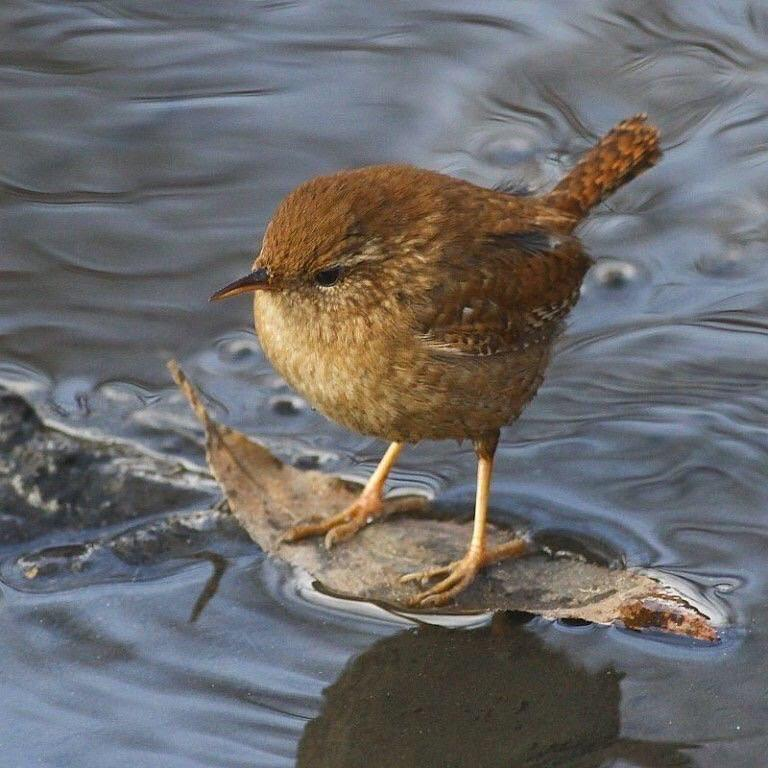
\includegraphics[width=0.5\linewidth]{figures/surfbird.jpg}
  \caption{
    \textbf{A surfing bird, looking very cool.} 
    After taking a few surfing lessons, William thought that maybe losing full custody of his kids wasn't that bad
  }
  \label{fig:1}
\end{figure}

\subsection{Doing this and that}
Blahblahblah. Here goes text. Blah. Do not read me~\cite{ExampleBook,ExampleArticle}.

\subsection{Doing it some more}
We will assess visionary need-to-knows within the core curriculum.


\subsection{And finally a crescendo of info}

Blahblahblhakjf.

\section{Conclusion}
By utilizing the excellent control over patch-patch attraction offered by the critical Casimir force, we experimentally explore some very nice physics.

\section{Methods}
\subsection*{Sample preparation}
We don't want to distract from our story with the methods, but actually this is like super important to understanding what we did~\cite{ExampleThesis}.

\bibliographystyle{unsrt}
\bibliography{bibliography}

\end{document}